\section{Object Design}
In questa fase si descrivono gli oggetti facenti parte del sistema e le componenti di terze parti utilizzate per la realizzazione del progetto.
\subsection{Componenti di Terze Parti}
PocketDev fa uso di varie librerie e tecnologie per la sua realizzazione:
\begin{itemize}
 \item Javascript: Linguaggio interpretato di scripting utilizzato per la realizzazione della logica di business e della pagina principale;
 \item HTML, CSS: Tencologie Web di base per la realizzazione di contenuti;
 \item KnockoutJS: Libreria per la realizzazione di interfacce dinamiche javascript tramite il pattern MVVM (Model-View-ViewModel);
 \item NodeJS: Ambiente per eseguire codice javascript al di fuori del browser; Presenta un'architettura di tipo Event-Driven ottima per gestire grossi carichi di lavoro;
 \item ExpressJS: libreria Javascript per Node utile per creare servizi REST in maniera semplice;
 \item Apache Fuseki: Funge da servizio per interrogare il database tramite SPARQL e serializzare il risultato in un formato compatibile per il web.
 \item TDB: Database che memorizze in formato efficiente triple in RDF;
 \item RDF: Sta per resource description framework e serve per descrivere la base di dati semantica tramite triplette di concetti;
 \item SPARQL: linguaggio per effettuare interrogazioni sul database semantico;
 \item Protégé: IDE grafico per la realizzazione dell'ontologia ideato dalla Stanford university;
\end{itemize}
\subsection{Diagramma delle classi}
\begin{figure}[H]
 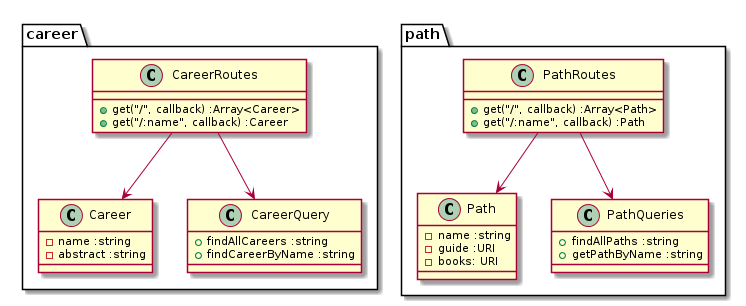
\includegraphics[scale=.5]{classdiagram.png}
\end{figure}
\subsection{Descrizione delle Query SPAQRL}
Di seguito sono riportate le query utilizzate per il prelevamento dei dati:
\subsubsection{Seleziona tutte le Carriere IT}
\begin{lstlisting}[language=SQL]
  SELECT ?name WHERE { 
  ?career a pd:IT_Career ;
  pd:hasName ?name .
}
\end{lstlisting}
La query preleva gli individui che sono del tipo IT\_Career e ne recupera la proprietà \textbf{hasName} e le restituisce. 
\subsubsection{Recupera percorso formativo teorico di una carriera}
\begin{lstlisting}
SELECT ?adv ?int ?bas WHERE {
  ?career a pd:IT_Career;
  pd:hasName ${name}.
  ?career pd:follow ?adv.
  ?adv pd:dependsOn ?int .
  ?int pd:dependsOn ?bas .
}
groupby ?adv ?int ?bas 
\end{lstlisting}
La query preleva la carriera tramite il suo nome univoco, recupera tutte le competenze teoriche avanzate di cui necessita e per inferenza si recuperano ricorsivamente con le ultime 2 triplette le conoscente intermedie e di base.
\subsubsection{Recupera percorso formativo pratico di una carriera}
\begin{lstlisting}
SELECT ?adv ?lib ?tool ?lang WHERE {
  ?carrer a pd:IT_Career ;
  pd:hasName ${name};
  pd:follow ?adv.
  ?adv rdf:type ?type.
  ?type rdfs:subClassOf* pd:Practice_EducationalPath.
  OPTIONAL {?adv pd:generate ?lib}
  OPTIONAL {?adv pd:usedWith ?tool}
}
\end{lstlisting}
La query preleva la carriera tramite il suo nome univoco, recupera tutti i concetti pratici che segue e recupera per inferenza le librerie e i tool. Per essere recuperati coerentemente utilizziamo la parola chiave optional all'interno delle triplette in quanto una carriera potrebbe avere necessitare solo di competenze pratiche di tipo Tool.
\subsubsection{Recupera informazioni concetto}
\begin{lstlisting}
SELECT ?type ?abs ?book ?guide WHERE {
  <${name}> rdf:type ?type .
  OPTIONAL  {<${name}> pd:hasBook ?book}
  OPTIONAL  {<${name}> pd:hasGuide ?guide}
  SERVICE <${endpoints.dbpedia}>{
    <${name}> dbo:abstract ?abs
  }
  FILTER (?type != owl:NamedIndividual)
  FILTER langMatches(lang(?abs),"en")
}
\end{lstlisting}
La query recupera il tipo, le info generiche, un url con l'insieme dei libri e la guida di uno specifico concetto teorico/pratico. Sia le condizioni per recuperare \textbf{hasBook} che \textbf{hasGuide} sono messe all'interno di una clausola optional perchè non le risorse esterne non forniscono libri e guide per tutti gli individui dell'ontologia. Poi la query si sposta sull'endpoint sparql messo a disposizione da DBPedia per recuperare l'abstract generale del concetto. il tutto viene filtrato selezionando unicamente contenuti in lingua inglese ed eliminando ridondanze di tipi. 
\subsection{Sviluppi Futuri}
Espandere l'ontologia può sicuramente arricchire la piattaforma con informazioni sempre più dettagliate e possibilmente eliminare lo scraper per avere una base di dati puramente semantica. Sarebbe anche utile poter associare anche i concetti pratici con quelli teorici in modo da avere un percorso formativo dal punto di vista pratico ancora più inerente alla carriera associata.
